\section{Overview}

This chapter describes the modeling pipeline used in this thesis, applied to the dataset described in \Cref{chap:dataset}: the attention-pooling classification architecture shared by all five encoder backbones (\Cref{sec:arch}); the centralized training procedure used to establish per-backbone baselines (\Cref{sec:centralized}); and the Flower/FedProx-based federated training pipeline used to simulate the privacy-preserving, cross-domain deployment scenario (\Cref{sec:federated}), including the infrastructure used and the practical implementation issues encountered. \Cref{fig:pipeline} summarizes the overall pipeline from the dataset (\Cref{chap:dataset}) to the ten trained models (five backbones $\times$ two training paradigms) evaluated in \Cref{chap:results}.

\begin{figure}[htbp]
    \centering
    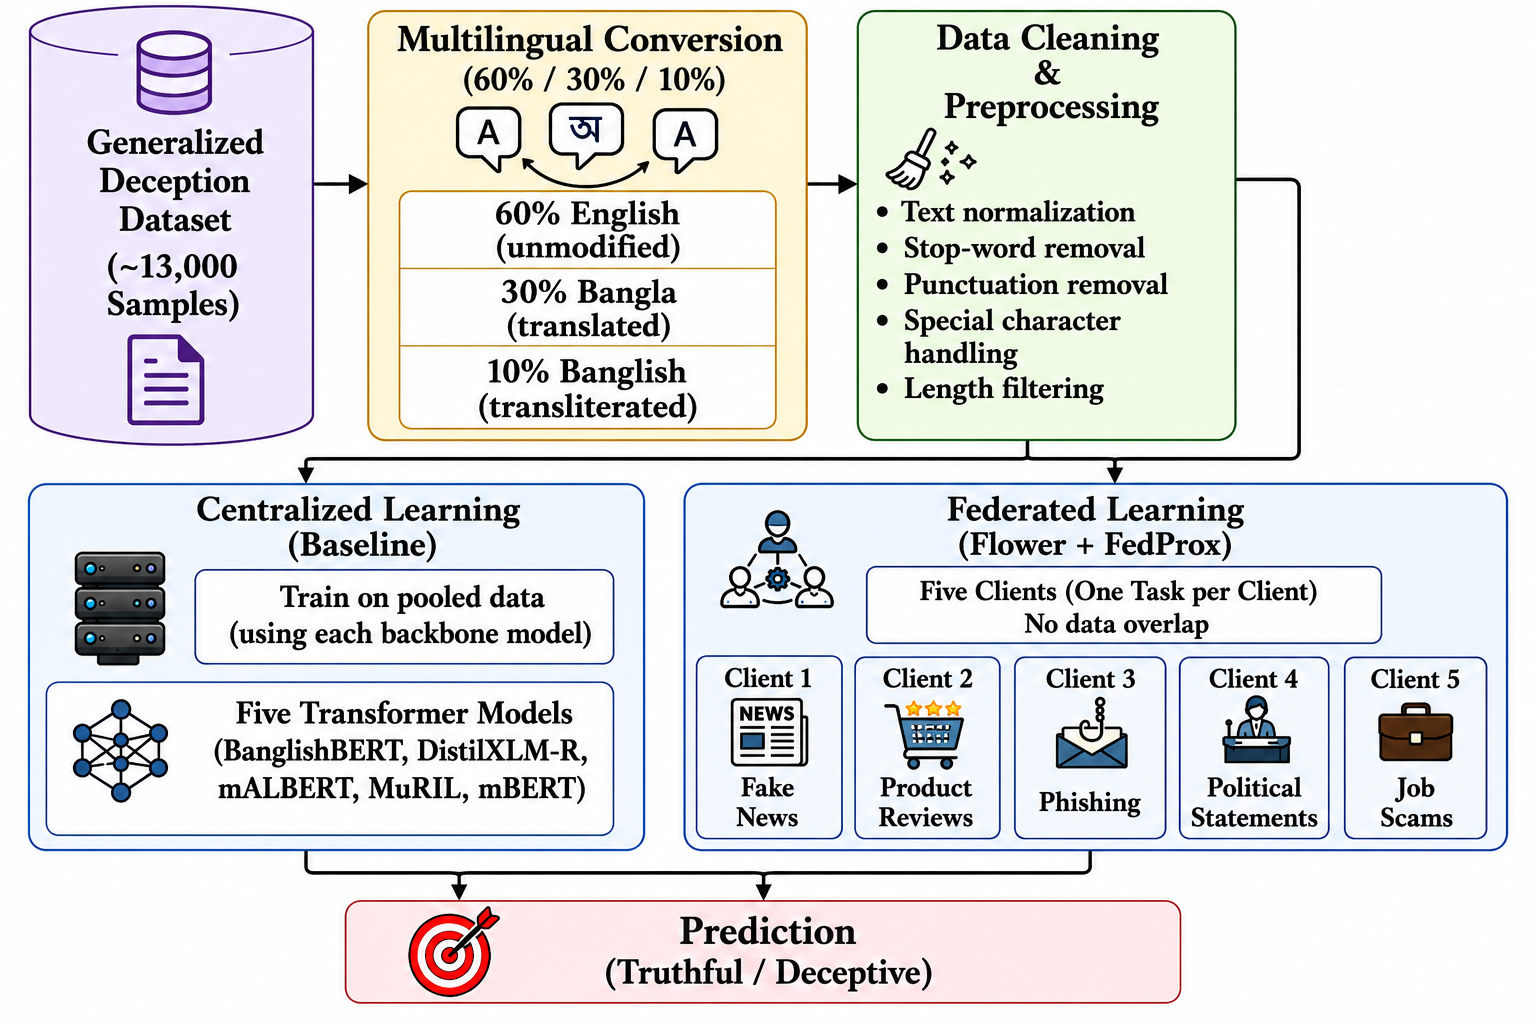
\includegraphics[width=\textwidth]{figures/overall_pipeline_F.png}
    \caption{Overall pipeline of the proposed multilingual deception detection framework.}
    \label{fig:pipeline}
\end{figure}

\section{Classification Architecture}
\label{sec:arch}

A single classification architecture is used across all five backbone encoders and both training paradigms, so that any difference in downstream performance can be attributed to the choice of backbone or training paradigm rather than to architectural differences in the classification head. 

\begin{figure}[htbp]
    \centering
    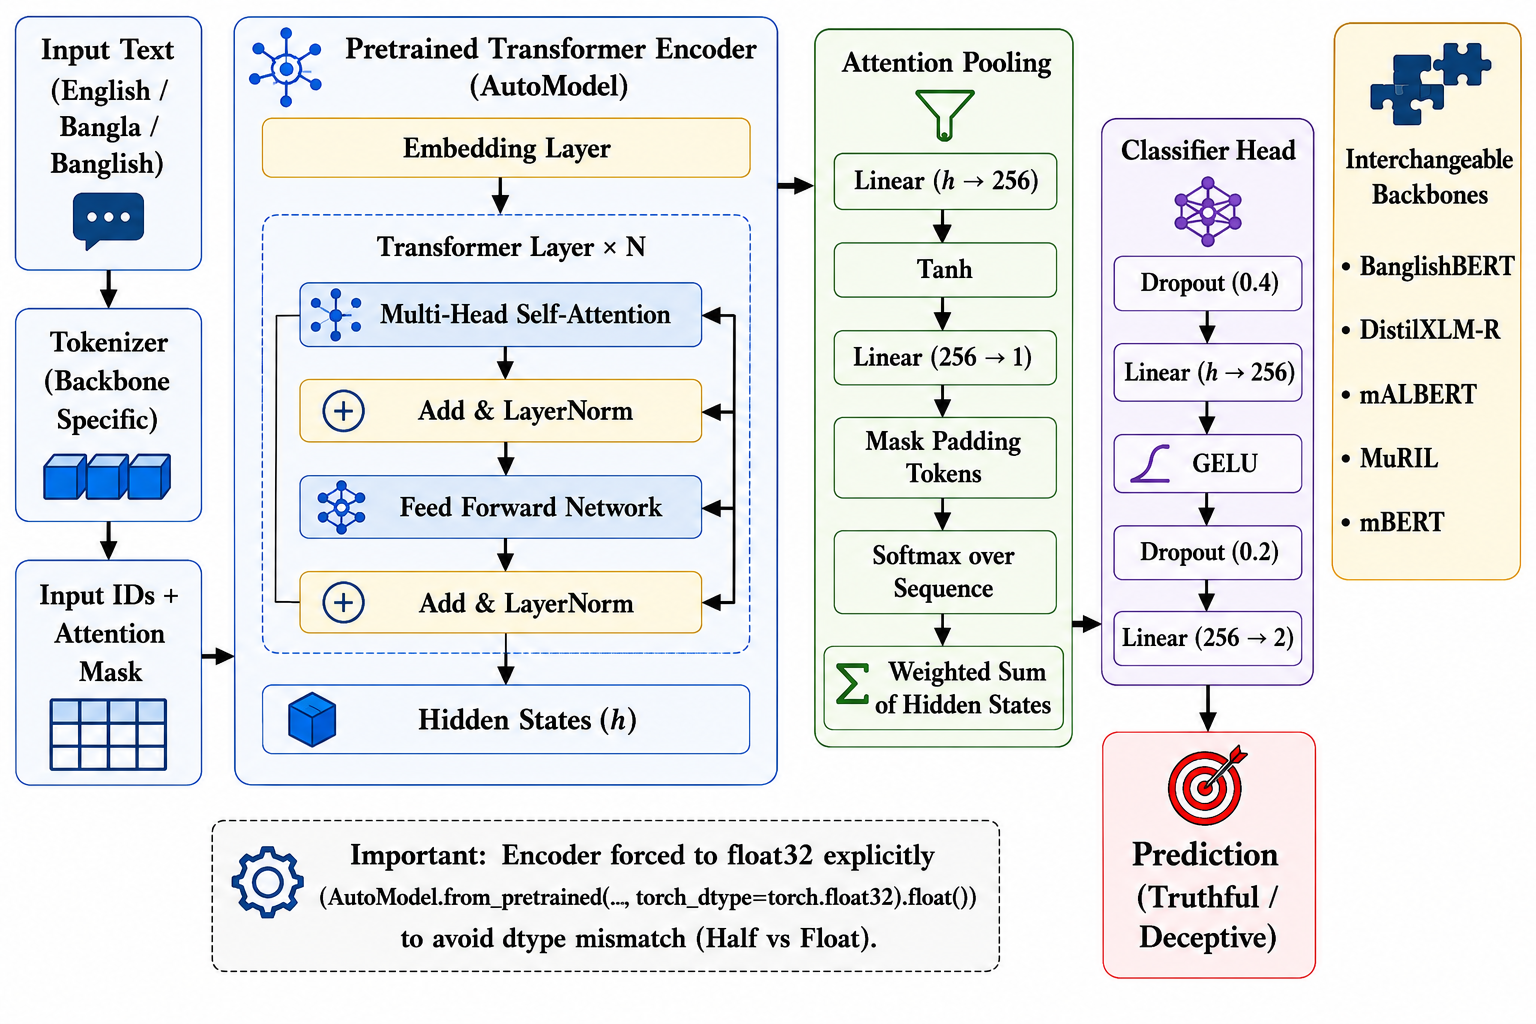
\includegraphics[width=0.95\textwidth]{figures/Transformer_architecture_F.png}
    \caption{Architecture of the proposed transformer-based text classification model. Input text is tokenized and encoded using a pretrained transformer backbone, followed by attention pooling and a fully connected classification layer to predict deceptive or truthful content. }
    \label{fig:transformer_architecture}
\end{figure}

\subsection{Tokenization and Encoding}

Input text is tokenized using the backbone-specific tokenizer (e.g.\ WordPiece for \gls{mbert}/\gls{muril}, SentencePiece for \gls{xlmr}) and passed through the corresponding pretrained Transformer encoder \cite{vaswani2017attention} (loaded via HuggingFace \texttt{AutoModel}), producing a sequence of contextual token embeddings of hidden size $h$ (backbone-dependent).

\subsection{Attention Pooling}

Rather than using the conventional \gls{cls} token representation as the pooled sequence embedding, this thesis uses a learned attention-pooling mechanism, which allows the model to weight informative tokens (e.g.\ hedging language, emotionally-charged words, or domain-specific red-flag phrases) more heavily than uninformative ones when forming the sequence-level representation used for classification:

\begin{enumerate}
    \item Each token's hidden state $h_i \in \mathbb{R}^{h}$ is scored by a two-layer network: $\text{Linear}(h \rightarrow 256) \rightarrow \tanh \rightarrow \text{Linear}(256 \rightarrow 1)$, producing a scalar attention score $e_i$ per token.
    \item Scores at padding-token positions are masked out (set to $-\infty$) before normalization.
    \item The scores are normalized across the sequence with a softmax to obtain attention weights $\alpha_i$.
    \item The pooled representation is the attention-weighted sum $z = \sum_i \alpha_i h_i$.
\end{enumerate}

\subsection{Classifier Head}

The pooled representation $z$ is passed through a classifier head: $\text{Dropout}(0.4) \rightarrow \text{Linear}(h \rightarrow 256) \rightarrow \text{GELU} \rightarrow \text{Dropout}(0.2) \rightarrow \text{Linear}(256 \rightarrow 2)$, producing the two class logits (truthful / deceptive). The two dropout layers (at rates 0.4 and 0.2) are intended to reduce overfitting given that several backbones are fine-tuned on a comparatively small, domain-partitioned slice of data in the federated setting.

\subsection{Precision Handling}

A practical implementation detail worth recording is that some HuggingFace Hub checkpoints (notably the distilled XLM-R checkpoint used as the DistilXLM-R backbone) ship with \texttt{fp16} weights by default. Loading such a checkpoint directly and combining it with the float32 classifier head above raises a dtype mismatch error (\texttt{mat1 and mat2 must have the same dtype, but got Half and Float}) during the first forward pass. This was resolved by explicitly forcing the encoder to \texttt{float32} at load time (\texttt{AutoModel.from\_pretrained(model\_name, torch\_dtype=torch.float32).float()}) for every backbone, ensuring numerically consistent and reproducible training across all five backbones.

\section{Backbone Encoders}
\label{sec:backbones}

Five multilingual or Bangla-aware pretrained encoders were evaluated as interchangeable backbones underneath the shared architecture of \Cref{sec:arch}, selected to span a range of multilingual strategies (general-purpose multilingual, Indian-language-specialized, Bangla-specialized) and model sizes (full-size vs.\ distilled/lite):

\begin{table}[htbp]
\centering
\caption{Backbone encoders evaluated in this thesis.}
\label{tab:backbones}
\begin{tabular}{@{}lp{7.2cm}l@{}}
\toprule
\textbf{Backbone} & \textbf{HuggingFace Checkpoint} & \textbf{Reference} \\
\midrule
mBERT & \path{google-bert/bert-base-multilingual-cased} & \cite{devlin2019bert} \\
DistilXLM-R & \path{nreimers/mMiniLMv2-L12-H384-distilled-from-XLMR-Large} & \cite{conneau2020xlmr, sanh2019distilbert} \\
MuRIL & \path{google/muril-base-cased} & \cite{khanuja2021muril} \\
BanglishBERT & \path{csebuetnlp/banglishbert} & \cite{bhattacharjee2022banglabert} \\
ALBERT Multilingual & \path{cservan/malbert-base-cased-32k} & \cite{lan2020albert} \\
\bottomrule
\end{tabular}
\end{table}

The XLM-R-family backbone used throughout this thesis, under both training paradigms, is \emph{DistilXLM-R} -- a distilled variant of XLM-R (\path{nreimers/mMiniLMv2-L12-H384-distilled-from-XLMR-Large}), chosen as a lightweight alternative that is well suited to the repeated local fine-tuning performed at each federated client while remaining tractable to also train centrally. Since no official distilled version of XLM-R has been released by its original authors, this MiniLM-based distillation of XLM-R-Large was selected as the closest publicly available equivalent while preserving multilingual representation capabilities. Because the identical checkpoint is used for both the centralized baseline (\Cref{sec:centralized}) and the federated run (\Cref{sec:federated}), DistilXLM-R forms a directly comparable matched pair, on equal footing with the other four backbones, for the accuracy-retention analysis in \Cref{sec:retention}.

\section{Centralized Training (Baseline)}
\label{sec:centralized}

For each backbone, a centralized baseline model is trained by fine-tuning the full architecture of \Cref{sec:arch} on the pooled (non-domain-partitioned) training split, using the entire training set in ordinary mini-batch gradient descent. This baseline establishes an upper-bound reference for how well each backbone can perform on this task when it is allowed unrestricted access to all training data at once, against which the federated results of \Cref{sec:federated} are compared.

\begin{table}[htbp]
\centering
\caption{Centralized training hyperparameters.}
\label{tab:central-hparams}
\begin{tabular}{@{}ll@{}}
\toprule
\textbf{Hyperparameter} & \textbf{Value} \\
\midrule
Optimizer & AdamW \\
Learning rate & $2 \times 10^{-5}$ \\
Batch size & 32 \\
Epochs & 10 \\
Maximum sequence length & 128 \\
Loss function & Cross-Entropy Loss \\
\bottomrule
\end{tabular}
\end{table}

\section{Federated Training}
\label{sec:federated}

\subsection{Federated Learning Setup}

The federated experiments simulate a realistic deployment in which each of the five deception domains (\Cref{chap:dataset}) is held by a separate, non-cooperating client that will not share its raw text with the server or with any other client. Training was implemented using the Flower federated learning framework \cite{beutel2020flower}, running in simulation mode with a Ray backend to orchestrate the five simulated clients. 

\begin{figure}[htbp]
    \centering
    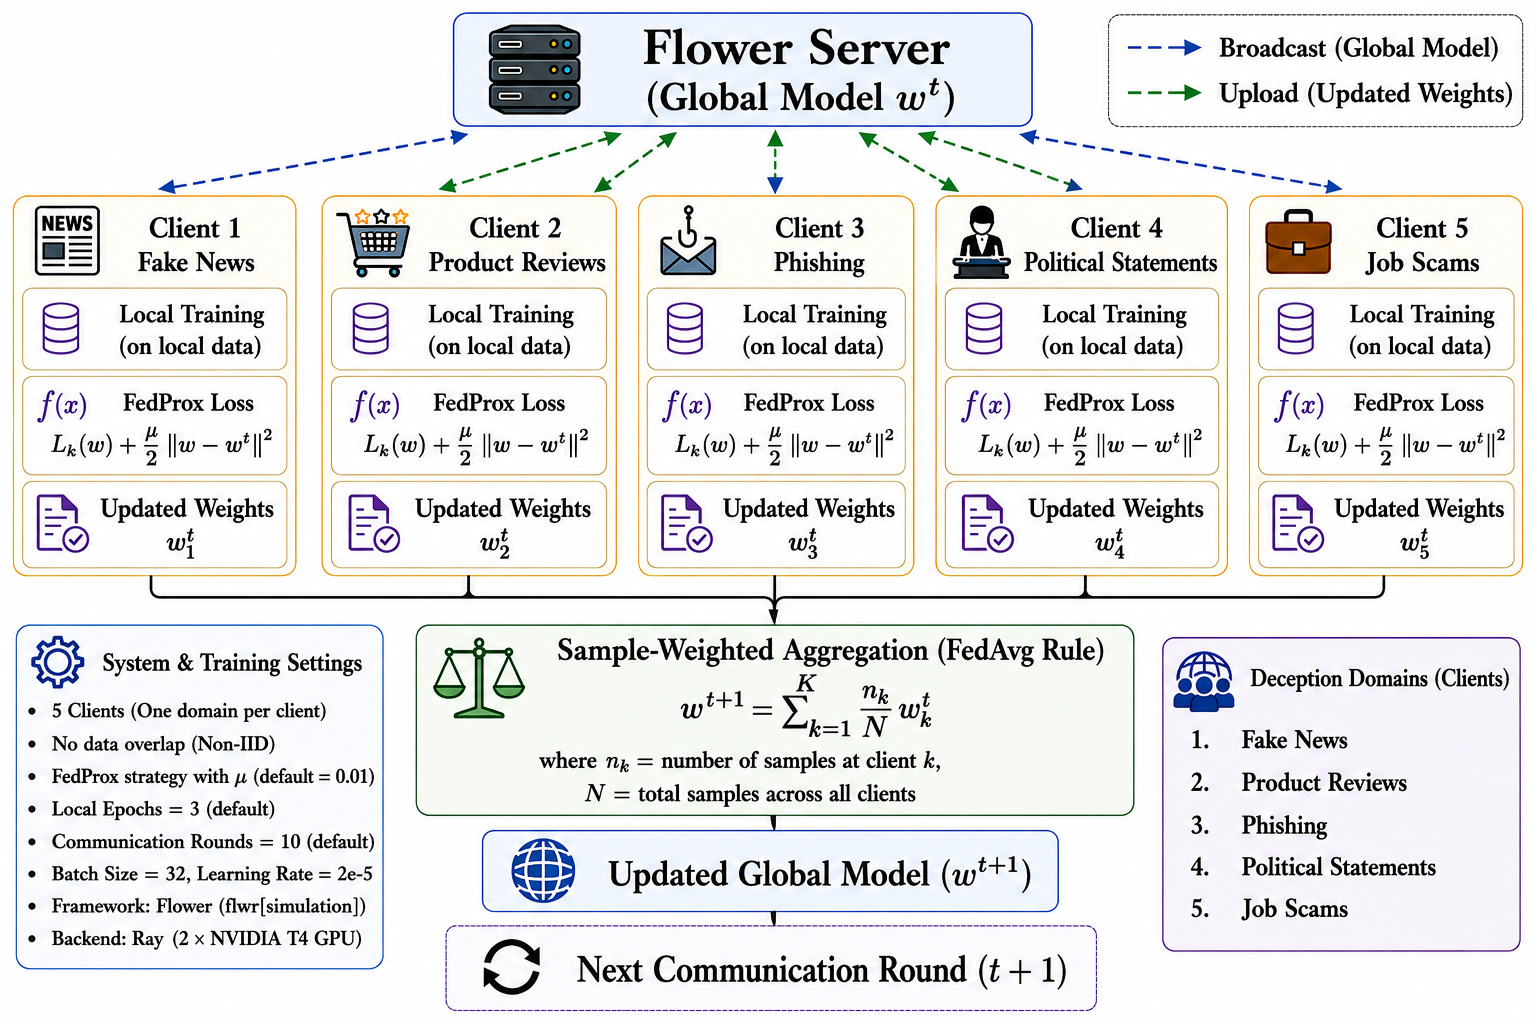
\includegraphics[width=0.95\textwidth]{figures/Federated_F.png}
    \caption{Architecture of the proposed federated learning framework. A central Flower server coordinates five federated clients, each representing a distinct deception domain.}
    \label{fig:federated_learning_architecture}
\end{figure}

\subsection{FedProx Optimization Strategy}

Because each client in this setting holds an entire, disjoint deception domain rather than a random subsample of a shared task, the resulting data heterogeneity across clients is considerably more severe than the (already non-trivial) heterogeneity typically assumed in the federated learning literature. Under such heterogeneity, plain \gls{fedavg} \cite{mcmahan2017communication} is known to suffer from client drift, where each client's locally-optimal model diverges substantially from the shared global objective between rounds of averaging. This thesis therefore adopts \gls{fedprox} \cite{li2020federated}, which modifies only the client-side local objective, leaving server-side aggregation unchanged:

\begin{equation}
L_k(w) = \ell_k(w) + \frac{\mu}{2}\lVert w - w^t \rVert^2
\end{equation}

where $\ell_k(w)$ is client $k$'s local cross-entropy loss, $w^t$ is a frozen snapshot of the global model parameters at the start of communication round $t$ (used only to compute the penalty, not updated during local training), and $\mu$ controls the strength of the proximal regularization pulling each client's local update back toward the global model. Server-side aggregation still follows the standard sample-weighted \gls{fedavg} rule,

\begin{equation}
w^{(t+1)} = \sum_{k=1}^{K} \frac{n_k}{n_{\text{total}}} \, w_k^{(t)},
\end{equation}

where $n_k$ is the number of training examples held by client $k$ and $n_{\text{total}} = \sum_k n_k$; \gls{fedprox} only changes what each client optimizes locally, not how the server combines the results.

\subsection{Federated Hyperparameters}

\begin{table}[htbp]
\centering
\caption{Federated (FedProx) training hyperparameters.}
\label{tab:fed-hparams}
\begin{tabular}{@{}ll@{}}
\toprule
\textbf{Hyperparameter} & \textbf{Value} \\
\midrule
Federated rounds (\texttt{FED\_ROUNDS}) & 10 \\
Local epochs per round (\texttt{LOCAL\_EPOCHS}) & 3 \\
Local batch size (\texttt{FED\_BATCH}) & 32 \\
Local learning rate (\texttt{FED\_LR}) & 2e-5 \\
Proximal term weight (\texttt{FEDPROX\_MU}) & 0.01 \\
Number of clients & 5 (one per deception domain) \\
Aggregation rule & Sample-weighted FedAvg (Eq.~2) \\
\bottomrule
\end{tabular}
\end{table}

The proximal weight $\mu = 0.01$ was used as the default operating point for the results reported in \Cref{chap:results}. Because the client partitioning in this thesis is unusually severe (each client holds one entire task/domain rather than a random subsample), a larger $\mu$ (in the range 0.1--1.0), combined with fewer local epochs per round and more communication rounds (e.g.\ \texttt{LOCAL\_EPOCHS}~=~1, \texttt{FED\_ROUNDS}~=~20), would be expected to reduce client drift further at the cost of additional communication overhead; this trade-off is left as a direction for future tuning (\Cref{chap:conclusion}) rather than explored exhaustively in this thesis.

\subsection{Infrastructure}

All experiments were run on Kaggle notebooks equipped with two NVIDIA T4 GPUs. The Flower simulation (\texttt{flwr[simulation]}) was configured with Ray as the backend, allocating a full GPU (\texttt{num\_gpus=1.0}) to each simulated client, so that two of the five clients trained concurrently on the two available GPUs during each round. Two practical issues were encountered and resolved during implementation:

\begin{enumerate}
    \item \textbf{Dependency resolution.} An initially pinned \texttt{ray==2.9.3} version was yanked from PyPI partway through development, breaking the environment build. This was resolved by relaxing the dependency specification to \path{flwr[simulation]>=1.8.0,<2.0}, allowing pip to resolve a currently-available compatible Ray version automatically.
    \item \textbf{Precision mismatch.} As described in \Cref{sec:arch}, some backbone checkpoints load in \texttt{fp16} by default, which is incompatible with the float32 classifier head; this was resolved by explicitly forcing every encoder to \texttt{float32} at load time.
\end{enumerate}

To tolerate the long-running nature of federated simulation on shared Kaggle compute, the pipeline checkpoints global model parameters after every communication round to \path{/kaggle/working/fed_checkpoints}. On restart, the pipeline computes the number of remaining rounds as \texttt{FED\_ROUNDS} minus the number of already-completed rounds (inferred from the latest checkpoint) and resumes federated training from that checkpoint as the \texttt{initial\_parameters} for the Flower strategy, rather than restarting from round zero.

\section{Evaluation Metrics}
\label{sec:metrics}

Every trained model (five backbones $\times$ two training paradigms) is evaluated on the same pooled test split (\Cref{chap:dataset}) using six metrics, reported together in \Cref{chap:results} rather than relying on accuracy alone, since domain-partitioned federated data carries a meaningful risk of class imbalance that accuracy alone can mask:

\begin{itemize}
    \item \textbf{Accuracy} -- overall proportion of correctly classified examples.
    \item \textbf{Precision} and \textbf{Recall} -- macro-averaged across the two classes.
    \item \textbf{Macro-F1 (\gls{f1})} -- the harmonic mean of macro-precision and macro-recall, more robust than accuracy under class imbalance.
    \item \textbf{\gls{auc}} -- the area under the ROC curve, measuring ranking quality independent of a fixed decision threshold.
    \item \textbf{\gls{mcc}} -- Matthews Correlation Coefficient, a single balanced measure computed from all four confusion-matrix cells that remains informative even under severe class imbalance.
\end{itemize}

In addition to these six per-model metrics, \Cref{chap:results} reports an \textbf{accuracy-retention} score, defined for any backbone for which both a centralized and a federated model were trained as

\begin{equation}
\text{Retention} = \frac{\text{Federated Accuracy (same backbone)}}{\text{Centralized Accuracy (same backbone)}} \times 100\%,
\end{equation}

which isolates the cost of moving from centralized to federated training for a fixed backbone, as distinct from the cost of choosing a weaker backbone -- a distinction that a bare comparison of federated and centralized numbers across \emph{different} backbones cannot make.

\section{Summary}

This chapter described the construction of a multilingual, five-domain deception detection dataset; a shared attention-pooling classification architecture used identically across five encoder backbones; a centralized training baseline; and a Flower/FedProx-based federated training pipeline designed around an unusually severe, task-partitioned form of client heterogeneity. The next chapter presents the resulting experimental performance of all trained models.
